\begin{figure*}[!t]
        \centering{
                \begin{tabular}{cccc}
                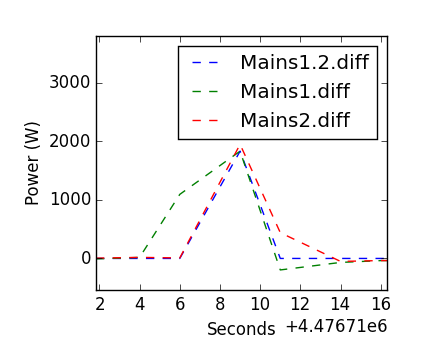
\includegraphics[width=3.2in]{multidisaggfig/dryerPhase12OnDiff.png} &
                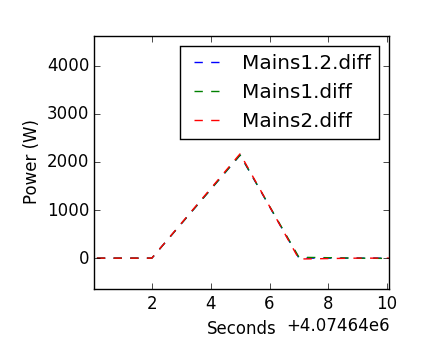
\includegraphics[width=3.2in]{multidisaggfig/waterHeaterPhase12OnDiff.png} \tabularnewline
                (a) & (b) \tabularnewline
                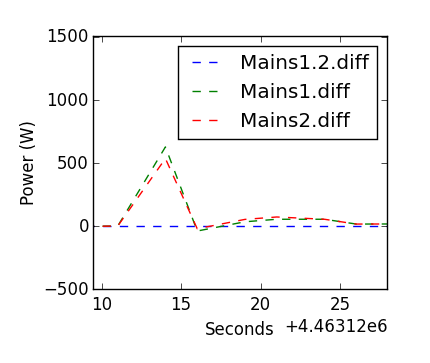
\includegraphics[width=3.2in]{multidisaggfig/heatingIndoorOutdoorPhase12On_1.png} &
                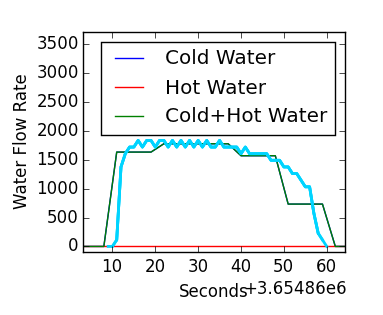
\includegraphics[width=3.2in]{multidisaggfig/UpToiletFitted.png}\tabularnewline
                (c) &(d) \tabularnewline
                \end{tabular}
                }
        \caption{
        Disaggregating dryer and continuous variable load heatingOutdoor with multivariate motif mining. The on event of a device and the corresponding diffs in the two phases for (a) dryer, (b) water heater, (c) heatingOutdoor. 
  	(d) Disaggregating the toilet water use end with dynamic time-warping subsequence search. This Y-axis is water flow rate in 10000*liter/minute.
        %(b) the diffs in two phases on event of water heater which shares same power level as dryer but different patterns when drawing power from two-phases.
       % (d) the disaggregated UpToilet of complete usage cycle by dynamic time warping subsequence search. This Y-axis is water flow rate in 10000*liter/minute.
        }
        \label{fig_dryerResults}
\end{figure*}
